\chapter{Liouville Geometry for Dissipative Systems}
\label{chap:contact_mechanics}
The contact-geometric counterpart of Hamiltonian and Lagrangian mechanics has been the subject of increasing academic interest in recent years, see for example \citet{VanderSchaft2021a,VanderSchaft2018,Maschke2018,Bravetti2017,DeLeon2020}, etc. The conception of the idea arguably traces back to the work of Herglotz \cite{Guenther1996}, who derived it using the variational principle, and the developments in differential geometry, by e.g. \citet{Arnold1989} and \citet{Libermann1987}.

In this chapter, the direct connection is made between the Caldirola-Kanai Hamiltonian given by \cref{eq:ham_CK} and the contact Hamiltonian described by \citet{Bravetti2017}, using Liouville geometry\footnote{It is interesting to note that Bravetti gives the Caldirola-Kanai method as an example of dissipative Hamiltonians in his paper, but fails to make the connection with his own method.}. We then proceed to \emph{contact Lagrangian mechanics}, strongly related to the Herglotz' work. Finally, the whole theory is explained from a thermodynamic perspective as well. While it was already known for some time (dating back to Arnol'd) that contact geometry is the preferred geometry for thermodynamics, its equivalence to contact geometry in (dissipative) classical mechanics has not been desribed in past literature. This underpins a famous statement by Vladimir Arnol'd that `contact geometry is all geometry', in the sense that conservative mechanical systems can be considered as part of a larger class of systems for which energy dissipation \emph{is} allowed. \cite{Geiges2008}

The traditional picture is that Hamiltonian mechanics takes place in the space of generalized positions and momenta, colloquialy denoted by $q$'s and $p$'s. The generalized positions form coordinates of the configuration manifold, which encodes all the possible positions that the system can find itself in. The momenta, on the other hand, are \emph{cotangent variables}: they live in the cotangent space of linear functions acting on tangent (velocity) vectors to the configuration manifold $Q$. We say that the Hamiltonian is a function on the \emph{cotangent bundle} to the configuration manifold $\ctbundle{Q}$. This cotangent bundle has a canonical `symplectic' structure, given by its symplectic form $\omega$, that pairs every position direction with its corresponding momenta:
$$ \omega = \sum \wedgep{\dd{q^i}}{\dd{p_i}}. $$
A vital property of symplectic manifolds (which include the cotangent bundle) is the fact that they are always even-dimensional: every position coordinate has a corresponding momentum and vice versa. Likewise, in an economic context this asserts that every product has its own price. It is precisely this symmetry that is broken by the introduction of contact manifolds.

The symplectic structure of Hamiltonian mechanics is related to the conservation of energy principle, The Hamiltonian function is conserved along the integral curves of the Hamiltonian vector field that it generates. For dissipative mechanics, this strict reciprocity between position and momentum is broken. Either, one constructs an explicit time-dependence and acknowledges the special nature of time, or one can introduce another coordinate that acts as `reservoir' to facilitate the dissipation in the system. These Hamiltonian systems are known as \emph{contact Hamiltonian systems}. One of the contributions of this thesis is to show how both methods are essentially equivalent, by connecting the most famous time-dependent model by Caldirola and Kanai to the contact Hamiltonian by \citet{Bravetti2017}.

\begin{figure}[ht!]
    \begin{center}
        \begin{tikzpicture}[every node/.style={outer sep=0pt,thick}]
    \tikzstyle{spring}=[thick,decorate,decoration={zigzag,pre length=0.3cm,post length=0.3cm,segment length=6}]
    \tikzstyle{damper}=[thick,decoration={markings,  
      mark connection node=dmp,
      mark=at position 0.5 with 
      {
        \node (dmp) [thick,inner sep=0pt,transform shape,rotate=-90,minimum width=15pt,minimum height=3pt,draw=none] {};
        \draw [thick] ($(dmp.north east)+(2pt,0)$) -- (dmp.south east) -- (dmp.south west) -- ($(dmp.north west)+(2pt,0)$);
        \draw [thick] ($(dmp.north)+(0,-5pt)$) -- ($(dmp.north)+(0,5pt)$);
      }
    }, decorate]
    \tikzstyle{ground}=[fill,pattern=north east lines,draw=none,minimum width=0.75cm,minimum height=0.3cm]

    \node (M) [draw,minimum width=1cm, minimum height=1.5cm] {$m$};

    \node (ground) [ground,anchor=north,yshift=-0.25cm,minimum width=1.5cm] at (M.south) {};
    \draw (ground.north east) -- (ground.north west);
    \draw [thick] (M.south west) ++ (0.2cm,-0.125cm) circle (0.125cm)  (M.south east) ++ (-0.2cm,-0.125cm) circle (0.125cm);

    \node (wall) [ground, rotate=-90, minimum width=2cm,yshift=-3cm] {};
    \draw (wall.north east) -- (wall.north west);

    \draw [spring] (wall.160) -- ($(M.north west)!(wall.160)!(M.south west)$) node[pos=0.5,anchor=south, outer sep=4pt] {$k$};
    \draw [damper] (wall.20) -- ($(M.north west)!(wall.20)!(M.south west)$) node[pos=0.5,anchor=north, outer sep=10pt] {$b$};

    \path (wall) ++(0.1cm, 1.2cm) -| node (q) {} (M);
    \draw[|->] (wall) ++(0.2cm, 1.2cm) -- (q.center) node[pos=0.5, anchor=south] {$q$};
    \draw (q) ++(0, 0.1cm) -- ++(0, -0.5cm);

    \node[bgelement] (J1) at (4.5, -1) {1};
    \node[bgelement, label=north:$k$] (C) at (4.5, 0.5) {C};
    \node[bgelement, label=east:$m$]  (I) at (6, -1) {I};
    \node[bgelement, label=west:$b$]  (R) at (3, 0.5) {R};

    % test
    \draw[bonds] 
        (J1) edge[e_out] (I)
        (J1) edge[f_out] (R)
        (J1) edge[f_out] (C);


\end{tikzpicture}

    \end{center}
    \caption{Schematic of the mass-spring-damper system.}
    \label{fig:dho}
\end{figure}
This chapter (and the application in the following chapter) is primarily concerned with the prototypical dissipative mechanical system: the linearly damped harmonic oscillator depicted in \cref{fig:dho}, with the governing second-order differential equation being
\begin{equation}  
  m\ddot{q} + b\dot{q} + kq = 0.
\end{equation}
The choice for this system is rather perspicuous, since it is arguably the `easiest' dissipative system that also exhibits second-order dynamics and is linear in all terms. Furthermore, as discussed below, it serves as the test case of choice in the overwhelming majority of research into dissipative Lagrangian and Hamiltonian mechanics
\cite{Dekker1981,Hutters2020b}. However, the method described in this section can be generalized directly to a general (possibly time-dependent) potential function $V = V(q, t)$. To make calculations and notation easier, some special parameters are frequently used throughout this chapter, they are summarized in \cref{tab:dho_params}.

\begin{table}[ht!]
    \caption{Parameter conventions of the damped harmonic oscillator. To avoid confusion with the symplectic form $\omega$, angular frequencies are denoted by $\Omega$ instead of the conventional lower case Greek letter.}
    \label{tab:dho_params}
    \begin{center}
        \begin{tabular}{llll}
            \toprule
            \textbf{Name} & \textbf{Symbol} & \textbf{Value} & \textbf{Units} \\
            \midrule
            Damping coefficient & $\gamma$ & $b/m$ & \si{\per \second }\\[0.4cm]
            Undamped frequency & $\Omega_o$ & $\sqrt{k/m}$ & \si{\per \second }\\[0.4cm]
            Damped frequency & $\Omega_d$ & $\sqrt{\Omega_0^2 - \qty(\frac{\gamma}{2})^2}$ & \si{\per \second }\\[0.4cm]  
            Damping ratio & $\zeta$ & $\frac{b}{2\sqrt{mk}}$ & -- \\[0.2cm]
            \bottomrule
        \end{tabular}
    \end{center}
\end{table}

\section{The Caldirola-Kanai method}
\label{sec:caldirola}
A traditional, engineering-inclined method to incorporate damping in the framework is to include a Rayleigh damping term in the Lagrangian to emulate linear damping forces, and this works `mathematically' to derive the correct equations of motion \cite{Goldstein2011}. Although frequently used for practical problems, this damping term is not really part of the \emph{actual} Lagrangian --- rather, it simply makes use of the notion of a generalized force that is not inherently part of the system. As such, this method only works on a superficial level: the pristine differential geometric foundations of mechanics do not leave room for such ad hoc tricks. There is, as a result, also no Hamiltonian counterpart for this method. 

The historical attempts to do better than the Rayleigh method were primarily motivated by the application of the (dissipative) Hamiltonian formalism in quantum mechanics through discretization. For this application, a sound mathematical structure is of the essence, which calls for a more rigorous approach. A celebrated paper by
\citet{Dekker1981} provides an excellent summary of many attempts up to 1981. Indeed, the well-studied approach developed by \citet{Caldirola1941} and \citet{Kanai1948} was intended exactly for this purpose. This method features an explicit time-dependence both in the Lagrangian function
\begin{equation}
    \Lck(q, \dot{q}, t) = \ec^{\gamma t}\qty(\frac{1}{2}m\dot{q}^2 - \frac{1}{2}kq_1^2),
    \label{eq:lag_CK}
\end{equation}
and the corresponding Hamiltonian function:
\begin{equation}
    \Hck(q, \Pcan, t) = \frac{\Pcan^2}{2m}\ec^{-\gamma t} + \frac{1}{2}kq^2\ec^{\gamma t}.
    \label{eq:ham_CK}
\end{equation}
In latter equation, $\Pcan$ refers to a special `canonical momentum', that is
\begin{equation}
    \Pcan \equiv \pdv{\Lck}{\dot{q}},
    \label{eq:can_momentum}
\end{equation}
which is related to the `true` kinematic momentum by the relation $\Pcan = p\ec^{\gamma
t} = m\dot{q}\ec^{\gamma t}$. As such, it is also clear that the Caldirola-Kanai Lagrangian and Hamiltonian functions are related by the Legendre transformation \emph{with respect to the canonical momentum}:
%\footnote{The `Legendre transform'
%refers, in the context of fiber bundles, to the so-called fiber derivative. On a manifold $M$, let $L \in
%\functions{M}$. Then the fiber derivative is defined als 
%    $$ \fiberder{L}: \tbundle{L}\to\ctbundle{L}: \fiberder{L}(\vec{v})\cdot\vec{w} = \left. \dv{}{s}\right\vert_{s = 0} L(\vec{v} +
%    s\vec{w}). $$
% Hence, the Legendre transformation is in the first place the mapping that associates the generalized velocities with the
% associated (canonical) generalized momenta. Importantly, this mapping is a diffeomorphism (that is, invertible and onto) if the Hessian of
% $L$ is nondegenerate - roughly equivalent to the statement that every generalized velocity has an associated `mass` to
% it. \cite{Marsden1998}}
$$ \Hck = \Pcan \dot{q} - \Lck. $$
From either \cref{eq:lag_CK} or \cref{eq:ham_CK}, the equations of motion are readily
derived (for the Hamiltonian case with respect to $\Pcan$ after which the transformation to $p$ can be effected).
Indeed, after taking the appropriate derivatives, one obtains:
\begin{equation*} 
    \begin{split}
        \dv{}{t}\qty(\pdv{\Lck}{\dot{q}}) - \pdv{\Lck}{q} &= 0 \\
        \Rightarrow \ec^{\gamma t}\qty(m\ddot{q} + m\gamma\dot{q} + kq) &= 0
    \end{split}
\end{equation*}
for the Lagrangian case. Likewise, Hamilton's equations yield: \cite{Tokieda2021}
\begin{equation*}
    \begin{split}
        \dot{q} &= \pdv{\Hck}{\Pcan} = \frac{\Pcan}{m}\ec^{-\gamma t} =  \frac{p}{m}, \\
        \dot{\Pcan} &= -\pdv{\Hck}{q} = -kq\ec^{\gamma t}.\\
    \end{split}
\end{equation*}
The relation between the time derivatives of the momenta $\dot{p}$ and $\dot{\Pcan}$ is slightly more involved since one must invoke the product rule as a result of their time-dependent relation:
\begin{equation}
    \dot{\Pcan} = \ec^{\gamma t}\qty(\dot{p} + \gamma p).  
    \label{eq:momentum_relation}
\end{equation}
Substition yields the correct equation for $p$, though the equation is again multiplied by $\ec^{\gamma t}$. Because the latter is sufficiently well-behaved (that is, it has no zeros), it can be removed without any problems.

\paragraph{Geometric perspective}
To put the above derivation in a geometric setting, define the Liouville 1-form as
$$ \alpha = \Pcan\dd{q} \quad \Rightarrow \quad \omega = -\dd{\alpha} = \wedgep{\dd{q}}{\dd{\Pcan}},$$
where the symplectic 2-form will be used to obtain Hamilton's equations. The Hamiltonian \cref{eq:ham_CK} is explicitly time-dependent. This will give rise to a time-dependent vector field governing the solution curves.\footnote
{A \emph{time-dependent vector field} on a manifold $M$ is a mapping $X: M\times\real \to \tbundle{M}$ such that for each $t \in \real$, the restriction $X_t$ of $X$ to $M \times \{t\}$ is a vector field on $M$. \cite{Libermann1987} An additional construction of importance, called the \emph{suspension} of the vector field, is a mapping $$ \tilde{X}: \real \times M \to \tbundle{(\real \times M)} \quad (t, m) \mapsto ((t, 1), (m, X(t, m))),$$ that is to say, it lifts the vector field to the extended space that also includes $t$ and assigns the time coordinate with a trivial velocity of 1. \cite{Abraham1978}}
The construction of the vector field associated with a time-dependent Hamiltonian follows the same construction rules as a normal Hamiltonian (using the isomorphism given by $\omega$), but `frozen' at each instant of $t$. Even more bluntly speaking, one simply ignores the $t$-coordinate during the derivation, only to acknowledge the dependence at the very end. This leads to the following vector field, `suspended' on the $\real\times Q$ space:
$$ \tilde{X}_{\Hck} = -\ec^{\gamma t}kq\pdv{}{\Pcan} + \ec^{-\gamma t}\frac{\Pcan}{m}\pdv{}{q} + \pdv{}{t}.$$
The suspension is important to make the final coordinate transformation from $\rho$ to $p$ work properly. Indeed, effecting the transformation $(q, \Pcan, t) \mapsto (q, \ec^{-\gamma t}\Pcan, t)$, one obtains
$$ \tilde{X}_{\Hck} = \qty(-kq - \gamma p)\pdv{}{p} + \frac{p_1}{m}\pdv{}{q} + \pdv{}{t}.$$
It is worthwile to ponder on some apparent peculiarities in the Caldirola-Kanai method, for they will be explained elegantly by the contact-Hamiltonian formalism. Firstly, the role of the two-different momenta is not very clear from the get-go, apart from being a consequence of the way the Caldirola-Kanai Lagrangian is formulated. This has also been the reason for considerable confusion in the academic community (see \citet{Schuch1997}). Furthermore, there is the special role of the time coordinate, which is merely a parameter in the Hamiltonian function; for it does not partake in the dynamics of the system. Finally, there is the special role of the factor $\ec^{\gamma t}$ through which the time-dependence makes its appearance both in the Lagrangian and the Hamiltonian.

%\section{Symplectification and Liouville structures}
%We start with an $n$-dimensional \emph{base manifold} $Q$. In the context mechanical systems, this manifold is the configuration manifold of the system, \emph{extended} with an additional, `special` position coordinate coordinate that will be interpreted later. Let us assume that $Q$ has coordinates $\vec{q} = \qty(q_0, q, \ldots, q_n)$. For the damped harmonic oscillator, this manifold is two-dimensional, for it contains just the special coordinate and the position of the mass. Without loss of generalization, we will denote the special position coordinate by $q_0$.
%
%Now, introduce the \emph{manifold of contact elements} $\cbundle{Q}$, to the base manifold $Q$. This is the manifold of all points in $Q$, with the space of all possible tangent hyperplanes at every point. This manifold has dimension $2n-1$.
%
%The manifold of contact elements to $Q$ can be identified with the projectivization of the cotangent bundle $\ctbundle{Q}$, denoted by $\pctbundle{Q}$. This manifold is of dimension $2n-1$. 

\section{From time-dependent to contact Hamiltonian systems}
In the subsequent discussion the original Hamiltonian will be progressively lifted to higher-dimensional spaces in order to include dissipation in the Hamiltonian formalism. First of all, to a contact manifold, which is odd-dimensional: as mentioned, we need an additional degree of freedom --- which has no momentum conjugate to it --- to keep track of the dissipation in the system. This degree of freedom is sometimes referred to as a \emph{gauge variable}, denoted by $q_0$.  However, performing calculations in contact geometry directly is cumbersome and uninsightful: to quote Vladimir Arnol'd once more, `one is advised to calculate symplectically but to think rather in contact geometry terms'. Hence, we make use of the \emph{symplectization} of the contact structure, which gives rise to a so-called \emph{Liouville structure}, and `pretend' that we are dealing with the symplectic case. This symplectization will add yet another dimension to the system. \cite{VanderSchaft2021a,Arnold1989a}

\subsection{Symplectization \& Liouville structures}
The contact manifold of our system is three-dimensional, with coordinates $p, q$ and $q_0$ -- the latter is the gauge variable for the dissipation in the system. It can be viewed as the manifold of contact elements associated with the extended configuration manifold $M$ for which $q$ and $q_0$ are coordinates, denoted by $\pctbundle{M}$. The contact form on $\pctbundle{M}$ is given by 
\begin{equation}
    \alpha = \dd{q}_0 - p\dd{q},
    \label{eq:dho_contact_form}
\end{equation}
which accentuates the special role of the $q_0$ in the system dynamics. Contact forms are, by their very nature, ambiguous: they represent a distribution of hyperplanes, which coincides with the kernel of the contact form. Multiplication with a nonzero factor yields a different contact form with the same kernel, that is to say, they represent the same contact structure. This is the reason behind the `projective' nature of contact mechanics\footnote{As explained in \cref{app:contact_geometry}, the manifold of contact elements is bundle-isomorphic to the projectivization of the cotangent bundle.}. Hence, one may just as well multiply the 1-form with a nonzero factor $\lambda$:
$$ \lambda\qty(\dd{q}_0 - p\dd{q}) \quad \lambda \in \real_0. $$
The factor $\lambda$ can be considered to be an extra degree of freedom (leaving the contact structure unaffected), which provides a `lift' from the odd-dimensional manifold to an even-dimensional one, which is called the symplectification of the contact manifold. \cite{Arnold1989}

To restate the above in canonical coordinates, choose\footnote
{The minus sign is there to obtain the convential form of the Liouville form in symplectic geometry.}
\begin{equation}
    \rho_0 = \lambda \quad \text{and} \quad \rho = -\lambda p
    \label{eq:homo_coords}
\end{equation}
such that
\begin{equation} 
    \theta = \rho_0\dd{q}_0 + \rho\dd{q}, 
    \label{eq:dho_liouville_form}
\end{equation}
which is the Liouville form on $\ctbundle{M}$. \cite[p. 308]{Libermann1987}  The Liouville form defines a symplectic structure given by\footnote
{The nondegeneracy condition on the contact structure guarantees that this structure is indeed symplectic.}
$$\omega = -\dd{\theta} = \wedgep{\dd{q_0}}{\dd{\rho_0}} + \wedgep{\dd{q}}{\dd{\rho}}.$$ 

\paragraph{Principal bundles}
Let us now formalize the Liouville structure in the language of principal bundles. The projectivized cotangent bundle $\pctbundle{M}$ has as its fiber the space of lines passing through the origin. These lines are also the orbits of the multiplicative group $\mgroup$ acting through dilations on the fiber of a bundle with two-dimensional fibers: the cotangent bundle of $M$ without zero section, denoted by $\ctzbundle{M}$. Using the canonical coordinates defined previously, coordinates for $\ctzbundle{M}$ are $(q_0, q, \rho_0, \rho)$, where $\rho$ and $\rho_0$ cannot vanish at the same time (the zero section). 
\begin{figure}[h!]
    \begin{center}
        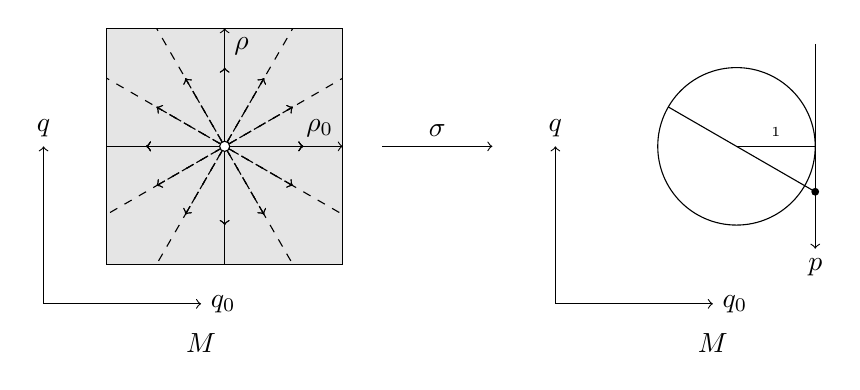
\begin{tikzpicture}
    \draw[->] (0, 0) -- (2, 0) node[anchor=west] {$q_0$};
    \draw[->] (0, 0) -- (0, 2) node[anchor=south] {$q$};
    
    \node (m) at (2.3, 2) {};
    
    \filldraw[draw=black, fill=gray!20] (m) ++(-1.5, -1.5) -- ++(0, 3) -- ++(3, 0) -- ++(0,-3) -- cycle;
    \draw[->] (m) ++(-1.5, 0) -- ++(3, 0) node[anchor=south east] {$\rho_0$};
    \draw[->] (m) ++(0, -1.5) -- ++(0, 3) node[anchor=north west] {$\rho$};
        
    \begin{scope}
        \clip (m) ++(-1.5,-1.5) rectangle ++(3, 3);
        \foreach \i in {0,30,...,180}{
            \draw[<->, dashed] (m) ++({-cos(\i)}, {-sin(\i)}) -- ++({2*cos(\i)}, {2*sin(\i)});
        }
        \foreach \i in {0,30,...,180}{
            \draw[<->, dashed] (m) ++({-cos(\i)}, {-sin(\i)}) -- ++({2*cos(\i)}, {2*sin(\i)});
        }
        \foreach \i in {0,30,...,180}{
            \draw[dashed] (m) ++({-4*cos(\i)}, {-4*sin(\i)}) -- ++({8*cos(\i)}, {8*sin(\i)});
        }
    \end{scope}
    
    \node[circle,draw=black,fill=white,inner sep=1.3pt] at (m) {};
    
    \draw[->] (6.5, 0) -- (8.5, 0) node[anchor=west] {$q_0$};
    \draw[->] (6.5, 0) -- (6.5, 2) node[anchor=south] {$q$};
    
    \node[fill=none] (m2) at (8.8, 2) {};
    
    \draw (m2) circle (1);
    \draw[->] (m2) ++(1, 1.3) -- ++(0, -2.6) node[anchor=north] {$p$} ;
    \draw (m2.center) ++(-0.866, 0.5) -- (9.8, 1.423) node[circle,fill=black, inner sep = 1pt] {};
    \draw (m2.center) -- ++(1, 0) node[pos=0.5,anchor=south] {\tiny{1}};
    %\draw[->] (m) ++(-1.5, 0) -- ++(3, 0) node[anchor=west] {$\rho_0$};
    %\draw[->] (m) ++(0, -1.5) -- ++(0, 3) node[anchor=south] {$\rho$};
    
    \draw[->] (4.3, 2) -- (5.7, 2) node[pos=0.5,anchor=south] {$\sigma$};
     
    \node at (2, -0.5) {$\ctzbundle{M}$};
    \node at (8.5, -0.5) {$\pctbundle{M}$};
\end{tikzpicture}

    \end{center}
    \caption{Illustration of the principal $\mgroup$-bundle $\bundle{\ctzbundle{M}}{\pi}{\pctbundle{M}}$. The total space $\ctzbundle{M}$ is the cotangent bundle to $M$ with zero section removed, which is shown on the left. The action by the multiplicative group $\mgroup$ is illustrated by the arrows, for it acts as a scaling (dilation) on all the cotangent variables. The origin is not part of the fiber, for it is part of the zero section. The bundle projection $\pi$ projects all points that are on the same orbit (straight lines through the origin) to a single point on the base manifold: the projectivized cotangent bundle $\pctbundle{M}$. The former space has a symplectic structure while the latter space has a contact structure. Observe from \cref{eq:homo_coords} that $p = \rho/\rho_0$, i.e. such that $p$ is a coordinate for the projectivization by stereographic projection, as shown on the right.}
    \label{fig:principal_bundle}
\end{figure}

Define the \mgroup-\emph{action} $\raction{}$ on $\ctzbundle{M}$ as:
$$ \raction: \ctzbundle{M}\times\mgroup \to \ctzbundle{M} : \quad (q_0, q, \rho_0, \rho) \blacktriangleleft \lambda = (q_0, q, \lambda \rho_0, \lambda \rho ) \qquad \lambda \in \mgroup,$$
which are referred to as dilations of the fiber.

As illustrated in \cref{fig:principal_bundle}, the \emph{orbit space} of $\ctzbundle{M}$ with respect to the group action $\raction{}$ is the space of all points in $\ctzbundle{M}$ with all points on the same line through the origin (in the fiber) identified. This space is precisely equal to the projectivization of the cotangent bundle $\pctbundle{M}$. Hence, consider the \emph{principal} $\mgroup$-bundle $\bundle{\ctzbundle{M}}{\sigma}{\pctbundle{M}}$ 
\begin{center}
    \begin{tikzcd}
        \ctzbundle{M} \\ \ctzbundle{M} \arrow[u, "\raction{\mgroup}"] \arrow[d, "\sigma"] \\ \pctbundle{M} \cong \cbundle{M}
    \end{tikzcd}
\end{center}
The removal of the zero section is required for the group action to be free. The principal bundle $\bundle{\ctzbundle{M}}{\pi}{\pctbundle{M}}$ admits a \emph{fibered symplectic Liouville structure}, given by the Liouville form \cite{Libermann1987}
$$ \theta = \rho_0\dd{q_0} + \rho\dd{q}, $$
and the associated two-form $\omega = -\dd{\theta}$. The distinctive feature of these forms that makes this a Liouville structure is that they both commute with the group action $\raction{}$: \cite{Libermann1987}
$$ (\raction{\lambda})^* \theta = \lambda \theta \qquad \lambda \in \real_*,$$
which makes them homogeneous forms of degree 1.

The projection map $\sigma$ of the principal bundle is locally defined as 
\begin{equation}
    \sigma : \ctzbundle{M} \to \pctbundle{M}: (q_0, q, \rho_0, \rho) \mapsto (q_0, q, -\rho/\rho_0), 
    \label{eq:principal_projection}
\end{equation}
with $p \equiv -\rho/\rho_0$ a coordinate for the projectivized fiber. This coordinate does not cover the entire fiber: the points for which $\rho_0 = 0$ is missing (in \cref{fig:principal_bundle}, this point is the only point on the circle that cannot be projected on the $p$-axis). However, we will make the deliberate assumption that in our application, $\rho_0$ is never equal to zero.
%The manifold $\ctzbundle{M}$ is called the symplectization of the contact manifold. For now, we have not assigned any specific meaning to the coordinates given above, but they will turn out to match with the notation used in \cref{eq:lag_CK,eq:ham_CK}, etc.

Finally, the \emph{Liouville vector field} $Z$ associated with the Liouville structure is the vector field that represents the dilation of the fiber in the symplectization. It is defined as
\begin{equation}
    Z = \fromDual{\omega}(\theta) = \rho_0\pdv{}{\rho_0} + \rho\pdv{}{\rho}. 
    \label{eq:liouville_vf}
\end{equation}
Vector field (components) colinear with the Liouville vector fields are called \emph{vertical}; they represent dissipative action in the system. After the vertical components are removed, they remaining vector field is called \emph{horizontal}.

[Liouville automorphisms, commute with the Liouville vector field -> very important in the chapter about split-quaternions]

To summarize, we lifted the original system with symplectic structure $\wedgep{\dd{q}}{\dd{p}}$ to a contact manifold through the addition of a gauge variable $q_0$. We then symplectified the contact manifold to a four-dimensional system, with `positions' $(q_0, q)$ and `momenta' $(\rho_0, \rho)$.

\begin{mathbox}{The importance of the zero section}
    Poincaré lemma, closed exact, Coen's form not holomorphic. \\
    You have to cheat somewhere to make this thing work. \\
    $$ \lied{X}{\omega} = \dd{\intpr{X}{\omega}} + \intpr{X}{\dd{\omega}} $$
    First form should be closed to make expression vanish, but is it also exact? Not on the same domain. Hamiltonian has a different domain than $ '\mathrm{d}' H $,
    i.e. forms are closed but not exact (on the entire domain), which is why you can't be on simply connected domain. \\
    $ \real^4 / \{(q_0, q, 0, 0)\} $ not simply connected
\end{mathbox}

\subsection{Homogeneous Hamiltonian systems} The theoretical construction of the past section serves an important purpose, because it is the symplectified space which is the proper setting for the Caldirola-Kanai Hamiltonian discussed in \cref{sec:caldirola}. Along with the symplectification of the contact structure described in the past section, we can do the same with a contact Hamiltonian system.

There is a one-to-one correspondence between contact Hamiltonians on $\pctbundle{M}$ and a special class of Hamiltonians on the symplectified space $\ctzbundle{M}$. These are the Hamiltonians which are \emph{homogeneous} in the cotangent variables with degree 1:\footnote
{This is a consequence of the Euler theorem for homogeneous functions. If $\mathscr{H} = \mathscr{H}(\vec{q}, \vec{\rho})$ is homogeneous of degree $r$ in $\vec{\rho}$, then
    $$ \sum_{i = 1}^n \rho_i \pdv{\mathscr{H}}{\rho_i} = r \mathscr{H}. $$
 Therefore, for homogeneity of degree 1, we have: 
 $$ \lied{Z}{\mathscr{H}} = Z(\mathscr{H}) = \sum_{i=1}^n \rho_i \pdv{\mathscr{H}}{\rho_i} = \mathscr{H} \quad \text{with}\quad Z \equiv \sum \rho_i \pdv{}{\rho_i}. $$
 The correspondence between the 
}
\begin{equation}
    \mathscr{H}(q_0, q, \lambda \rho_0, \lambda \rho) = \lambda\,\mathscr{H}(q_0, q, \rho_0, \rho) \quad \text{or} \quad \lied{Z}{\mathscr{H}} = \mathscr{H},
\end{equation}
with $\lambda \in \real_0,\: H \in \functions{\ctzbundle{M}}$ and $Z$ defined according to \cref{eq:liouville_vf}. Given that $H$ is indeed homogeneous of degree 1, this correspondence is in canonical coordinates:
\begin{equation}
    \mathscr{H}(q_0, q, \rho_0, \rho) = -\rho_0\,H\qty(q_0, q, -\frac{\rho}{\rho_0})
    \label{eq:H_correspondence}
\end{equation}
where $\mathscr{H} \in \functions{\ctzbundle{M}}$, $H \in \functions{\pctbundle{M}}$ and $p = -\rho / \rho_0$ is a coordinate for the projectivized fiber. Likewise, there is also a direct correspondence between the vector fields generated by these Hamiltonians, and therefore the system dynamics. This is the reason why we go through the trouble of symplectification in the first place, it offers significant computational advantages. It is possible to derive the contact equations directly (as \citet{Bravetti2017} does), but it does not offer the same amount of insight as its symplectified counterpart. \cite{VanderSchaft2021a,Arnold1989}

Now, recall the Caldirola-Kanai Hamiltonian in \cref{eq:ham_CK}. Instead of assuming a direct time-dependence, we will think of the time-dependence as the gauge momentum, i.e. $\rho_0 = -\ec^{\gamma t}$. However, we will now consider $\rho_0$ to be a coordinate in its own right, instead of directly using the expression above. The Caldirola-Kanai Hamiltonian is then written as (cf. \cref{eq:ham_CK}):
$$ \Hck = -\rho_0 \qty[\frac{1}{2m}\qty(-\frac{\rho}{\rho_0})^2 + \frac{1}{2}kq^2]. $$
The motivation to make this particular choice is twofold: first, observe that $\mathscr{H}$ is homogeneous in the cotangent variables $\rho_0, \rho$, and second, that their fraction yields the \emph{real} momentum: $ p = -\rho/\rho_0 $. However, we must acknowledge a potential dependence on $q_0$, since we want to convert the explicitly time-dependent Hamiltonian into a contact Hamiltonian. We therefore add the arbitrary function $f(q_0)$, whos value is to be determined later, and also multiply by $\rho_0$ to maintain homogeneity. Denote the homogeneous Hamiltonian by $\mathscr{H}$:
\begin{equation}
    \mathscr{H}: \ctzbundle{M} \to \real: \quad \mathscr{H}(q_0, q, \rho_0, \rho) = -\rho_0 \qty[\frac{1}{2m}\qty(-\frac{\rho}{\rho_0})^2 + \frac{1}{2}kq^2 + f(q_0)]. 
    \label{eq:homo_hck}
\end{equation}
 Using the correspondence given by \cref{eq:H_correspondence}, the homogeneous Hamiltonian may be `projected' to the contact Hamiltonian $H$:
\begin{equation}
    H: \pctbundle{M} \to \real: \quad H(q_0, q, p) = \frac{p^2}{2m} + \frac{1}{2}kq^2 + f(q_0).
\end{equation}
Numerically, this contact Hamiltonian is the same as the Hamiltonian for an undamped mass-spring system but it is defined on the contact manifold that also takes into account the gauge variable $q_0$.

\emph{Equations of motion} Now to derive the equations of motion. As mentioned, this is easiest in the symplectified space because Hamilton's equations can be readily applied (the reader can consult \cref{app:contact_geometry} for the direct derivation). Because we are using canonical coordinates, the Hamiltonian vector field
\begin{equation}
    X_\mathscr{H} = \fromDual{\omega}(\dd{\mathscr{H}})
    \label{eq:ham_vf}
\end{equation}
corresponds to Hamilton's equations in the familiar form:
\begin{equation}
    \dv{\rho}{t} = -\pdv{\mathscr{H}}{q},\quad
        \dv{\rho_0}{t} = -\pdv{\mathscr{H}}{q_0},\quad
        \dv{q}{t} = \pdv{\mathscr{H}}{\rho},\quad
        \dv{q_0}{t} = \pdv{\mathscr{H}}{\rho_0}.
\end{equation}
Observe that this motivates why one has to take the partial with respect to the `other' momentum in the Caldirola-Kanai momentum: we are dealing with a specific instance of a more general class of homogeneous coordinates of the cotangent variables. Of course, the variable of interest is the actual momentum $p$, not the scaled version $\rho$. The time-derivative of $p$ can be written in terms of $\rho$ and $\rho_0$, completely analogous to \cref{eq:momentum_relation}:
\begin{equation}
    p = -\rho/\rho_0 \quad\Rightarrow\quad \dv{p}{t} = -\frac{1}{\rho_0}\dv{\rho}{t} + \frac{\rho}{\rho_0^2}\dv{\rho_0}{t} = -\frac{1}{\rho_0}\dv{\rho}{t} - \frac{p}{\rho_0}\dv{\rho_0}{t}. 
    \label{eq:homo_momenta}
\end{equation}
Given \cref{eq:homo_hck}, the partial derivatives of $\mathscr{H}$ and $H$ are related through the by relations: \cite{Arnold1989}
\begin{equation}
    \begin{split}
        \pdv{\mathscr{H}}{q} &= -\rho_0 \pdv{H}{q}, \\
        \pdv{\mathscr{H}}{q_0} &= -\rho_0 \pdv{H}{q_0}, \\
        \pdv{\mathscr{H}}{\rho} &= -\rho_0 \pdv{H}{p}\pdv{p}{\rho} = \pdv{H}{p}, \\
        \pdv{\mathscr{H}}{\rho_0} &= -H - \rho_0 \pdv{H}{p}\pdv{p}{\rho_0} = -H - \pdv{H}{p}\frac{\rho}{\rho_0} = \pdv{H}{p}p - H.\\
    \end{split}
    \label{eq:partial_relation}
\end{equation}
Hence, the \emph{contact} equations of motion can be found by combining of \cref{eq:momentum_relation} and \cref{eq:partial_relation}:
\begin{equation}
    \begin{split}
        \dv{q}{t} &= \pdv{H}{p} \\
        \dv{p}{t} &= \frac{1}{\rho_0}\pdv{\mathscr{H}}{q} + \frac{p}{\rho_0}\pdv{\mathscr{H}}{q_0} = - \pdv{H}{q} - p\pdv{H}{q_0} \\
        \dv{q_0}{t} &= \pdv{H}{p}p - H.
    \end{split}
    \label{eq:contact_eom}
\end{equation}
Some observations are important to note:
\begin{itemize}
    \item The evolution of the position $q$ remains the same as for the `normal' (undamped) case.
    \item The evolution of the momentum operator picks up a term that is depends on presence of the gauge variable in the contact Hamiltonian.
    \item The evolution of the gauge variable is equal to the Legendre transformation of the contact Hamiltonian with respect to $p$.
\end{itemize}

We are now ready to determine the nature of the as of yet unknown function $f$ to obtain the correct equations of motion. By comparing \cref{eq:homo_momenta} and \cref{eq:contact_eom}, the following relation must hold:
$$ \frac{1}{\rho_0}\dv{\rho_0}{t} = \pdv{H}{q_0} = \dv{f}{q_0}. $$
Furthermore, since we initial `substituted' $\ec^{\gamma t}$ in favor of $\rho_0$, the left hand side of the equation should be equal to $\gamma$ for it to be consistent with the Caldirola-Kanai Hamiltonian. Hence, we know that $\dv{f}{q_0} = \gamma$, or $f(q_0) = \gamma q_0$ up to a constant, which we choose to be zero. Although this may seem like an odd construction, the only thing we did is made the contact equation of motions equivalent with the time-dependent equations of motion. Now, the fact that $\rho_0 = \ec^{\gamma t}$, ceases to be an a priori assumption, and is derivable through Hamilton's equations:
$$ \dv{\rho_0}{t} = -\pdv{\mathscr{H}} = \gamma\rho_0 \quad \Rightarrow \quad \rho_0 = \ec^{\gamma t} + C$$

As such, we have for the contact Hamiltonian:
\begin{equation}
    H: \pctbundle{M} \to \real: \quad H(q_0, q, p) = \frac{p^2}{2m} + \frac{1}{2}kq^2 + \gamma q_0,
    \label{eq:H_dho}
\end{equation}
and this is precisely Bravetti's result. For the homogenous Hamiltonian on the symplectified space, we have:
\begin{equation}
    \mathscr{H}: \ctzbundle{M} \to \real: \quad \mathscr{H}(q_0, q, \rho_0, \rho) = -\rho_0\,\qty[\frac{1}{2m}\qty(-\frac{\rho}{\rho_0})^2 + \frac{1}{2}kq^2 + \gamma q_0]. 
    \label{eq:H_dho_homo}
\end{equation}
%It is easily verified that the contact Hamilton equations $\cref{eq:contact_eom}$ yield the correct equations of motion for the damped harmonic oscillator:
%$$ \dv{q}{t} = p/m \qquad \dv{p}{t} = -kq -\gamma p.$$
%On the other hand, the equation of motion for $q_0$ requires some additional considerations; this is the subject of the next section.

The Hamiltonian vector field $X_\mathscr{H} \in \vfields{\ctzbundle{M}}$ is then, using \cref{eq:H_dho_homo} and \cref{eq:ham_vf}:
$$ X_{\mathscr{H}} = \frac{p}{2m}\pdv{}{q}\: + \: \qty[\frac{1}{2m}\qty(\frac{\rho}{\rho_0})^2 - \frac{1}{2}kq^2]\pdv{}{q_0}\: + \: \rho_0 kq \pdv{}{\rho}\: + \: \gamma \rho_0 \pdv{}{\rho_0}.$$ 

The contact Hamiltonian vector field $X_H \in \vfields{\pctbundle{M}}$ is obtained either by using the contact Hamilton equations given by \cref{eq:contact_eom}, or by using the pushforward of the projection map $\sigma$:
$$ X_H = \sigma_*\,X_\mathscr{H} = \frac{p}{2m}\pdv{}{q}\: + \: \qty(\frac{p^2}{2m} - \frac{1}{2}kq^2)\pdv{}{q_0}\: - \: (kq + \gamma p)\pdv{}{p}\: $$
This is essentially the equivalent of the time-dependent transformation performed in \cref{sec:caldirola}. Clearly, these yield the correct equations of motion for the damped harmonic oscillator.

\paragraph{Mehcanical energy} One of the computational advantages of the symplectified space is the fact that `regular' Poisson brackets can be used in contrast to their slightly unwieldy contact counterparts. Define therefore a lift that takes functions from the contact manifold to the symplectified manifold:
$$ 
    \ell : \functions{\pctbundle{M}} \to \functions{\ctzbundle{M}}: \quad g \mapsto g \circ \sigma,
$$
with $\sigma$ as in \cref{eq:principal_projection}. The function takes the same value but is expressed in terms of the coordinates of the symplectified space.

The mechanical energy, denoted by $E$, is equal to 
$$ E(q_0, q, p) = \frac{p^2}{2m} + \frac{1}{2}kq^2,$$
which can be lifted to the symplectified space
$$ 
    \ell(E)(q_0, q, \rho_0, \rho) = \frac{1}{2m}\qty(-\frac{\rho}{\rho_0})^2 + \frac{1}{2}kq^2.
$$
The change of mechanical energy in the system is then readily determined using the Poisson brackets:
$$ \dv{E}{t} = \poisson{\mathscr{H}}{\ell(E)} = \lied{X_\mathscr{H}}{\ell(E)} = \frac{\gamma}{2m}\qty(\frac{\rho}{\rho_0})^2 = \frac{\gamma}{2m}p^2,$$
which is precisely the dissipative power in the damping element.

\subsection{Interpretation of the canonical variables}
Another advantage of using the purely symplectic formalism on the lifted space is the fact that the homogeneous Hamiltonian is invariant under the flow it generates, since the explicit time-dependence has been removed:
$$ \dv{\mathscr{H}}{t} = \poisson{\mathscr{H}}{\mathscr{H}} = \lied{X_{\mathscr{H}}}{\mathscr{H}} = 0. $$
We may therefore associate the homogeneous Hamiltonian with a constant. By inspection of \cref{eq:H_correspondence}, 
$$ \mathscr{H} = -\rho_0\,\underbrace{\qty(C\rho_0^{-1})}_{H} \qquad C \in \real.$$
Recall that we made the assumption earlier that $\rho_0$ is a function \emph{without zeros}. 

The constant $C$ is a degree of freedom in the system that we are free to choose, for the equations of motion will be consistent with any chosen value. This called a \emph{gauge} of the system, and its choice will influence the value of the gauge variable directly. The contact Hamiltonian is not a constant of motion however (at least, for dissipative systems). With some abuse of notation
$$ \dv{H}{t} = C\,\dv{\rho_0}{t}  = -C\,\pdv{\mathscr{H}}{q_0}.$$
Until now, there were no assumptions regarding the value of the damping constant $\gamma$: indeed, the `normal' equations of motion are readily derived when $\gamma$ is set to zero. We will now add the assumption that there is at least some dissipation present in the system ($\gamma \neq 0$) to assign further intrepretation to the gauge variable. The evolution of $q_0$ is directly related to the evolution of $H$ by \cref{eq:H_dho}
$$ q_0 = \frac{1}{\gamma} \qty(\rho_0 C - E). $$
Because we are free to choose the value of $C$, let us now make a choice of particular interest; namely $C = 0$. In that case, both $\mathscr{H}$ and $H$ vanish \emph{weakly};\footnote
{The weak equality, as opposed to the strong equality, is not maintained under variations. Hence, although the numerical value of the function is zero, its partial derivatives do not necessarily vanish. The reader is referred to \citet{Dirac1950} for a more elaborate discussion.}
this choice rids us from the additional freedom in $C$ that would also show up in the equation of motion for $q_0$. Instead, $q_0 = - E/\gamma$; which can be interpreted as the heat dissipated by the system (one can add a suitable initial condition for $q_0(0) = E(0)$ to make this also numerically correct). The vanishing of the Hamiltonians reflect the energy balance that is maintained throughout the evolution of the system:
$$ H = E + Q $$
We can also make a canonical transformation from

!! jet bundles for higher-dimensional systems

\section{Legendre involution}
In the classic, symplectic case, the Legendre transformation is used to pass from the Hamiltonian to the Lagrangian formalism and vice versa. This is because the Legendre transform facilitates a mapping between the tangent and cotangent bundle. If the Lagrangian (or Hamiltonian) is (hyper)regular (i.e. the mass matrix is invertible), this mapping is a diffeomorphism. \cite{Carinena1990}

One would be tempted to use the normal Legendre transformation on the symplectified Hamiltonian $\mathscr{H}$. This approach will meet some problems though:
\begin{itemize}
    \item A homogeneous function is not regular in the homogeneous variables --- naturally, a degree of freedom still resides in the action of the multiplicative group. Therefore, the mapping from the cotangent to the tangent bundle is not a diffeomorphism. Said otherwise, there is not a one-to-one correspondence between the homogeneous momenta and the associated velocities in the Lagrangian description.
    \item As a consequence of Euler's theorem for homogeneous functions, the Legendre transformation for a homogeneous function is necessarily equal to zero. For any homogeneous function $H$ (of degree 1), Euler's theorem states that
    $$ \sum_{i = 1}^n \rho_i \pdv{\mathscr{H}}{\rho_i} = \mathscr{H}, $$

        i.e. the function is equal to its associated `action', and therefore the expression for the Legendre transformation vanishes. \cite{Dirac1950,Dirac1933}
\end{itemize}
There is a better path to take. In essence the Legendre transform is (and was originally meant to be) a \emph{contact transformation}.

